\documentclass[a4paper]{article}
\usepackage{ctex}
\usepackage{geometry}
\usepackage{amsmath}
\usepackage{ulem}
\usepackage{graphicx}
\usepackage{siunitx}
\usepackage{enumitem}
\usepackage{multirow}
\usepackage{adjustbox}
\usepackage[hidelinks]{hyperref}
\usepackage{tabularx}
\usepackage{array}
\usepackage{float}
\usepackage[siunitx]{circuitikz}
\newcolumntype{Y}{>{\centering\arraybackslash}X}

\geometry{left=2.5cm, right=2.5cm, top=2.5cm, bottom=2.5cm}
\zihao{-4}

\begin{document}

\noindent\textbf{班级：24级整合科学班} \hspace{1cm} \textbf{学号：2400017802} \hspace{1cm} \textbf{姓名：冯翊展} \hspace{1cm} \textbf{评分：}\\
\textbf{同组学生：胡家豪} \\
\textbf{实验名称：滤波器与温度监测电路 }   \hfill \textbf{实验日期：2025年5月16日} 

\hrule
\vspace{3mm}

\begin{enumerate}[label=\chinese*.,left=0pt]
    \item 实验目的
    \begin{enumerate}[label=\arabic*.,left=0pt]
        \item 使用电阻和电容制作滤波器，并利用信号发生器和示波器测量频率响应。
        \item 使用热敏电阻和 NI DAQ制作温度监测电路，并用LabVIEW读取信号，绘制温度曲线图。
    \end{enumerate}
    
    \item 基本原理
    \begin{enumerate}[label=\arabic*.,left=0pt]
        \begin{figure}[H]
            \centering
            \begin{minipage}{0.6\textwidth}
                \centering
                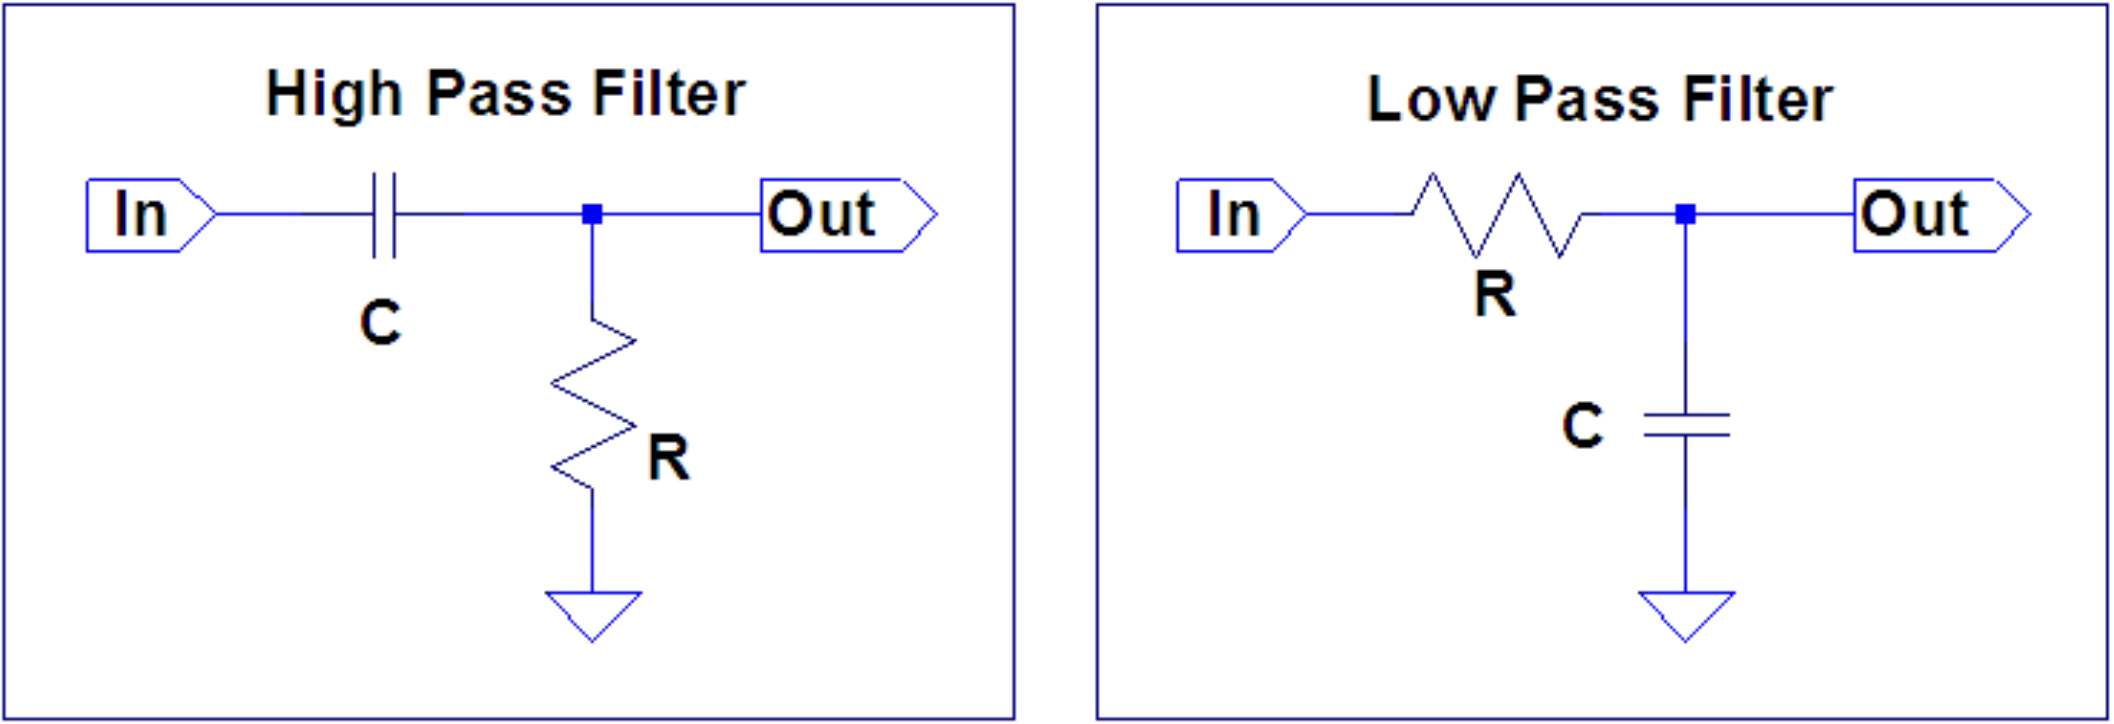
\includegraphics[width=\textwidth]{Filter.png}
            \end{minipage}
            \begin{minipage}{0.3\textwidth}
                \centering
                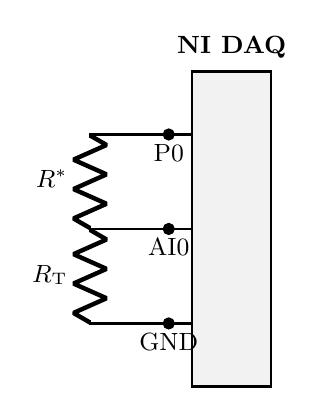
\begin{tikzpicture}[font=\small, pin distance=1.2cm, node distance=1cm]
                    \draw[thick, fill=gray!10] (0,0) rectangle (1,4);
                    \node at (0.5,4.3) {\textbf{NI DAQ}};

                    \filldraw[black] (-0.3,3.2) circle (2pt);
                    \draw[thick] (-0.3,3.2) -- (0,3.2);
                    \node[below] at (-0.3,3.2) {P0};

                    \filldraw[black] (-0.3,2.0) circle (2pt);
                    \draw[thick] (-0.3,2.0) -- (0,2.0);
                    \node[below] at (-0.3,2.0) {AI0};

                    \filldraw[black] (-0.3,0.8) circle (2pt);
                    \draw[thick] (-0.3,0.8) -- (0,0.8);
                    \node[below] at (-0.3,0.8) {GND};

                    \draw[thick] (-0.3,3.2) to (-1.3,3.2) to[R, l_=$R^*$] (-1.3,2.0) to (-0.3,2.0);
                    \draw[thick] (-1.3,2.0) to[R, l_=$R_\text{T}$] (-1.3,0.8) to (-0.3,0.8);
                \end{tikzpicture}
            \end{minipage}
            \caption{滤波电路和温度监测电路}
        \end{figure}
        \item 滤波电路 
        \\[1mm]
        以高通滤波器为例，电容$C$的阻抗为 $Z_C = -j/\omega C$，故
        $$ I = \frac{V_{\text{in}}}{Z_{\text{total}}}= \frac{V_{\text{in}}}{R - j / \omega C}= \frac{V_{\text{in}} (R + j / \omega C)}{R^2 + 1 / \omega^2 C^2} $$
        $$V_{\text{out}} = IR = \frac{V_{\text{in}} R (R + j / \omega C)}{R^2 + 1 / \omega^2 C^2}$$ 
        $$|V_{\text{out}}| = \left(V_{\text{out}}V_{\text{out}}^*\right)^{1/2} = \frac{V_{\text{in}} R}{\left[R^2 + (1/{\omega^2 C^2})\right]^{1/2}} = \frac{2 \pi f RC}{\left[1 + (2 \pi f RC)^2 \right]^{1/2}} V_{\text{in}}$$
        同理，对于低通滤波器，
        $$|V_{\text{out}}| = \frac{1}{\left[1 + (2 \pi f RC)^2 \right]^{1/2}} V_{\text{in}}$$
        两种电路的截止频率均为 $f_{\text{3dB}} = 1/2\pi RC$。

        \item 温度监测电路
        \\[1mm]
        电路如图所示，DAQ P0为数字信号输出端口，设置输出1时提供 $V_0=\qty{3.4}{\V}$，AI0为模拟信号输入端口，测量输入电压，GND 为接地端口；$R^*$ 为定值电阻，$R_\text{T}$ 为热敏电阻，其工作曲线满足
        $$\ln \frac{R_\text{T}}{R_0} = B \left(\frac{1}{T}-\frac{1}{T_0}\right)。$$
        由此可得温度-电压关系：
        $$T = \left[\frac{1}{T_0}+\frac{1}{B} \ln\left(\frac{R^*}{R_0} \frac{V}{V_0-V}\right)\right]^{-1}。$$

    \end{enumerate}
    \item 仪器与试剂
    \\[3mm]
    面包板，导线，电阻，热敏电阻，电容，万用表，信号发生器，示波器，NI DAQ，电脑

    \item 实验步骤
    \begin{enumerate}[label=\arabic*., left=0pt]
        \item 选取合适的电阻与电容，使用万用表测量其参数；组合成高通或低通滤波电路，使用信号发生器和示波器测量其频率响应并与理论曲线拟合。重复五组实验。
        \item 使用LabVIEW读取示波器波形，并利用GUI实现对示波器的控制。
        \item 使用热敏电阻组装温度监测电路，建立热敏电阻工作曲线，使用LabVIEW绘制15分钟温度变化曲线。
    \end{enumerate}
    
    \item 实验结果与分析
    \begin{enumerate}[label=\arabic*.,left=0pt]
        \item 滤波电路
        \\[1mm]
        选取5种电阻-电容组合，在面包板上连接高通和低通滤波电路。使用信号发生器作为信号输入，示波器接受信号输出。调整信号发生器产生的正弦波频率，记录示波器信号响应，绘图并与理论图像比较，结果如下（左为高通滤波，右为低通滤波）：
        \begin{figure}[H]
            \centering
            \scalebox{0.8}{
            \begin{minipage}{0.45\textwidth}
                \centering
                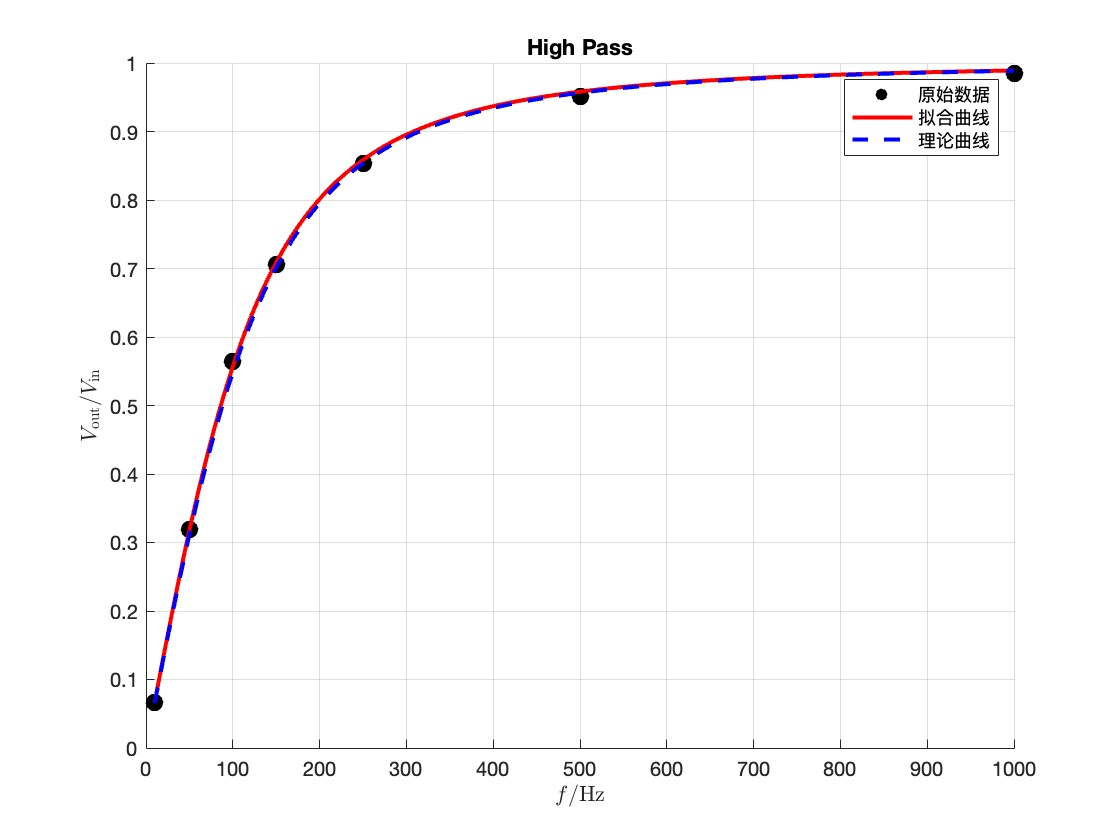
\includegraphics[width=\textwidth]{RC1H.jpg}
            \end{minipage}
            \begin{minipage}{0.45\textwidth}
                \centering
                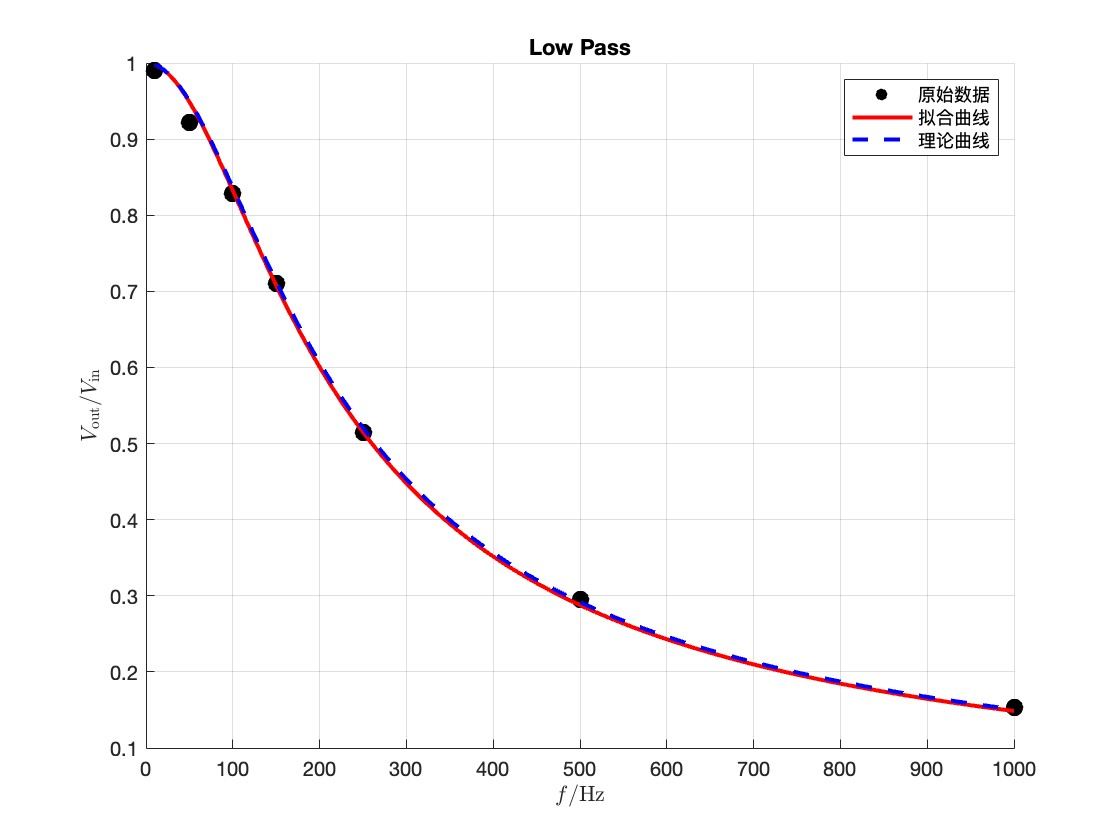
\includegraphics[width=\textwidth]{RC1L.jpg}
            \end{minipage}
            }
            \caption{$R=\qty{9.9}{\kohm}$，$C=\qty{105.4}{\nF}$}
        \end{figure}
        \begin{figure}[H]
            \centering
            \scalebox{0.8}{
            \begin{minipage}{0.45\textwidth}
                \centering
                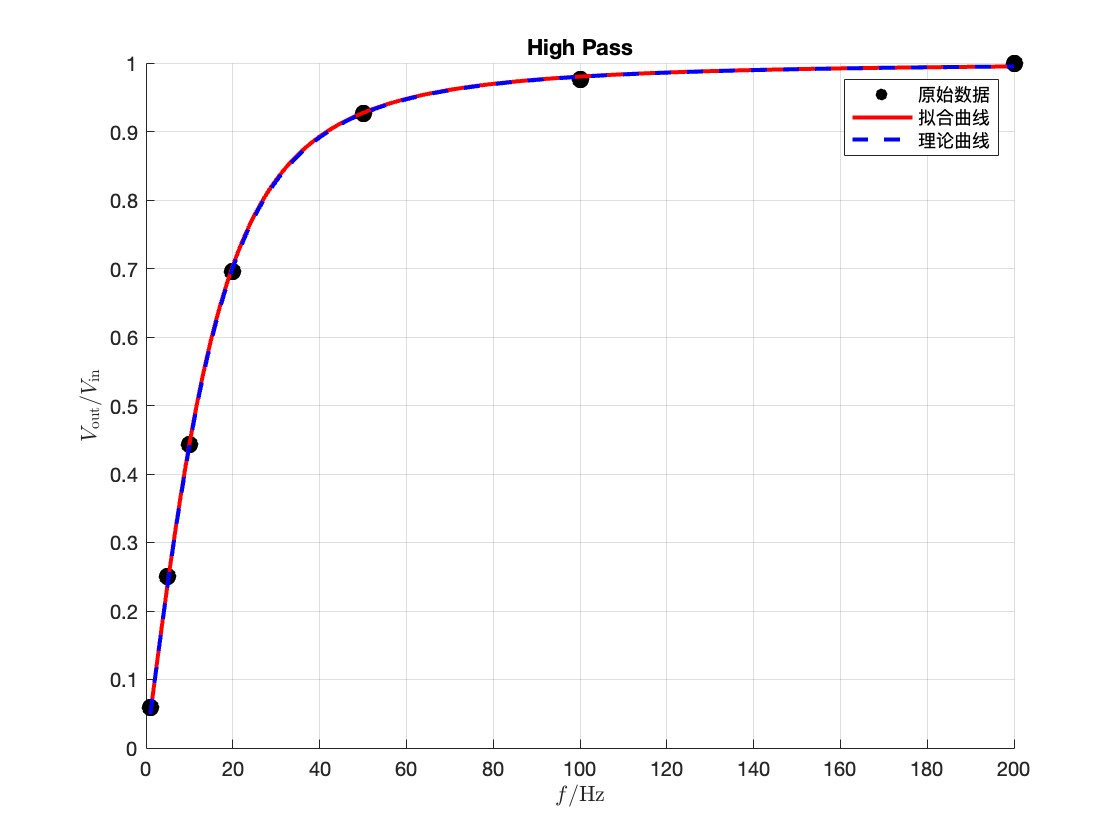
\includegraphics[width=\textwidth]{RC2H.jpg}
            \end{minipage}
            \begin{minipage}{0.45\textwidth}
                \centering
                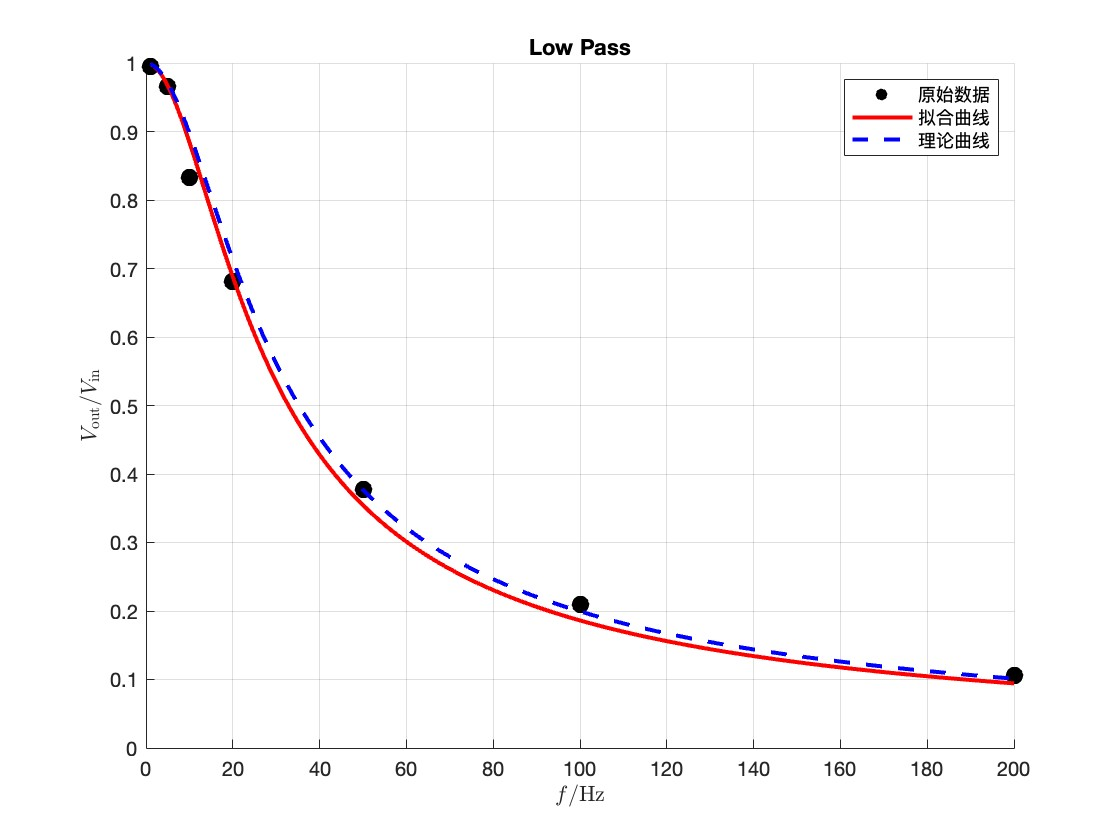
\includegraphics[width=\textwidth]{RC2L.jpg}
            \end{minipage}
            }
            \caption{$R=\qty{74.2}{\kohm}$，$C=\qty{105.4}{\nF}$}
        \end{figure}
        \begin{figure}[H]
            \centering
            \scalebox{0.8}{
            \begin{minipage}{0.45\textwidth}
                \centering
                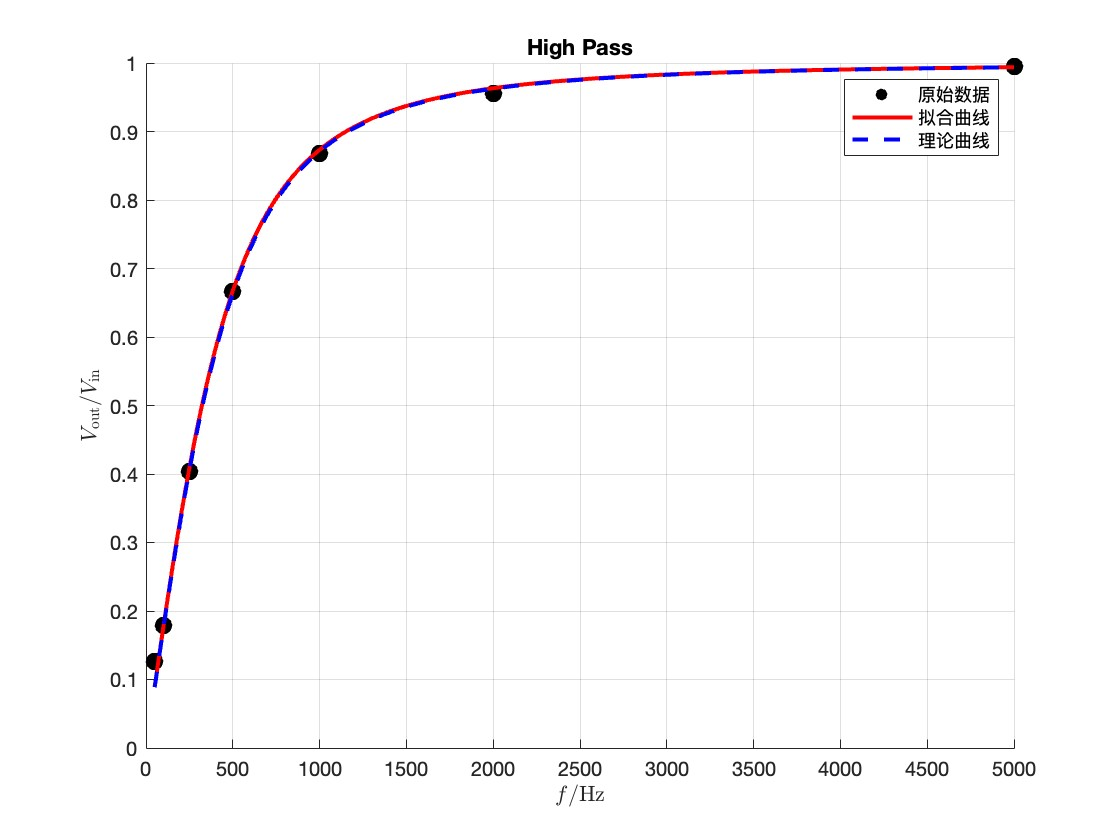
\includegraphics[width=\textwidth]{RC3H.jpg}
            \end{minipage}
            \begin{minipage}{0.45\textwidth}
                \centering
                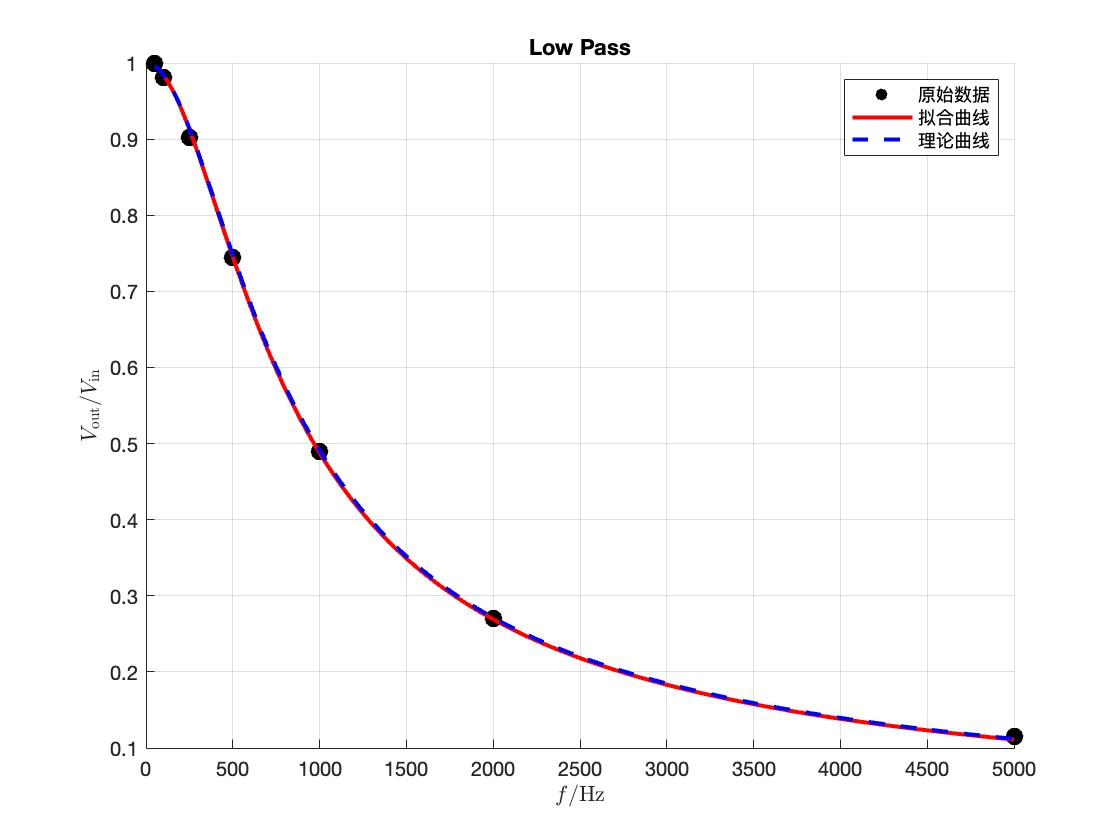
\includegraphics[width=\textwidth]{RC3L.jpg}
            \end{minipage}
            }
            \caption{$R=\qty{2.678}{\kohm}$，$C=\qty{105.4}{\nF}$}
        \end{figure}
        \begin{figure}[H]
            \centering
            \scalebox{0.8}{
            \begin{minipage}{0.45\textwidth}
                \centering
                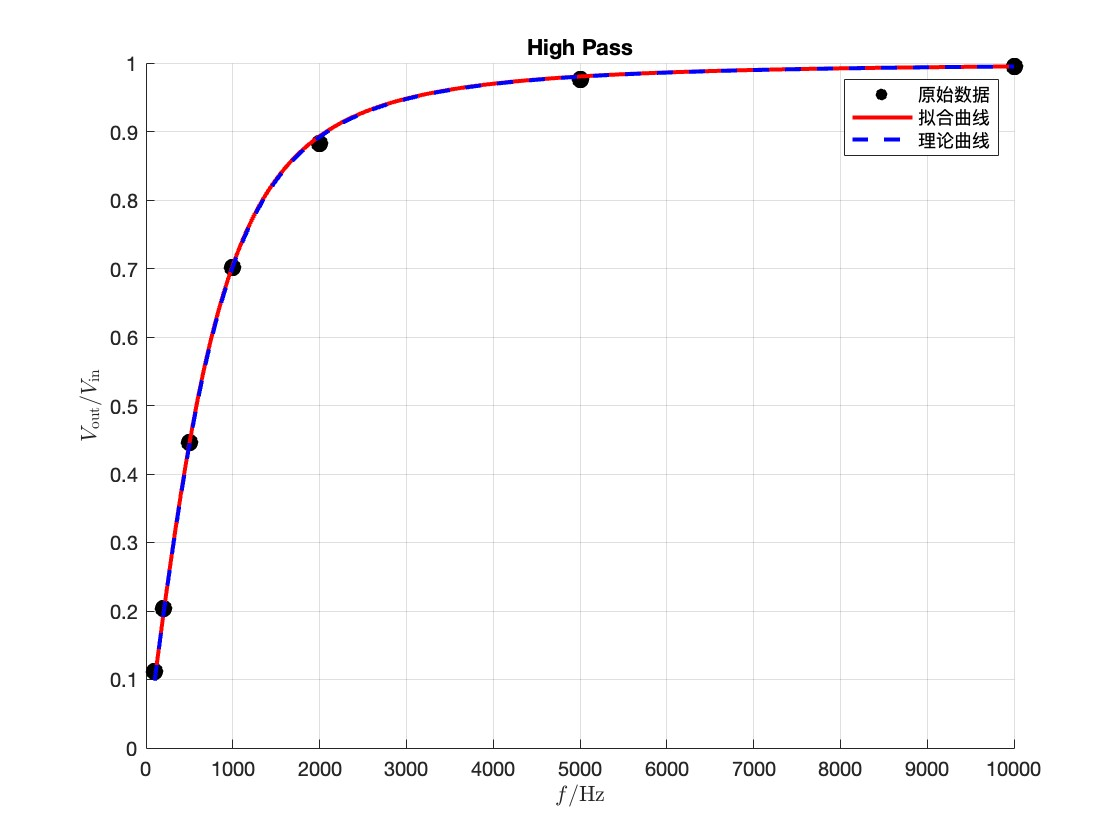
\includegraphics[width=\textwidth]{RC4H.jpg}
            \end{minipage}
            \begin{minipage}{0.45\textwidth}
                \centering
                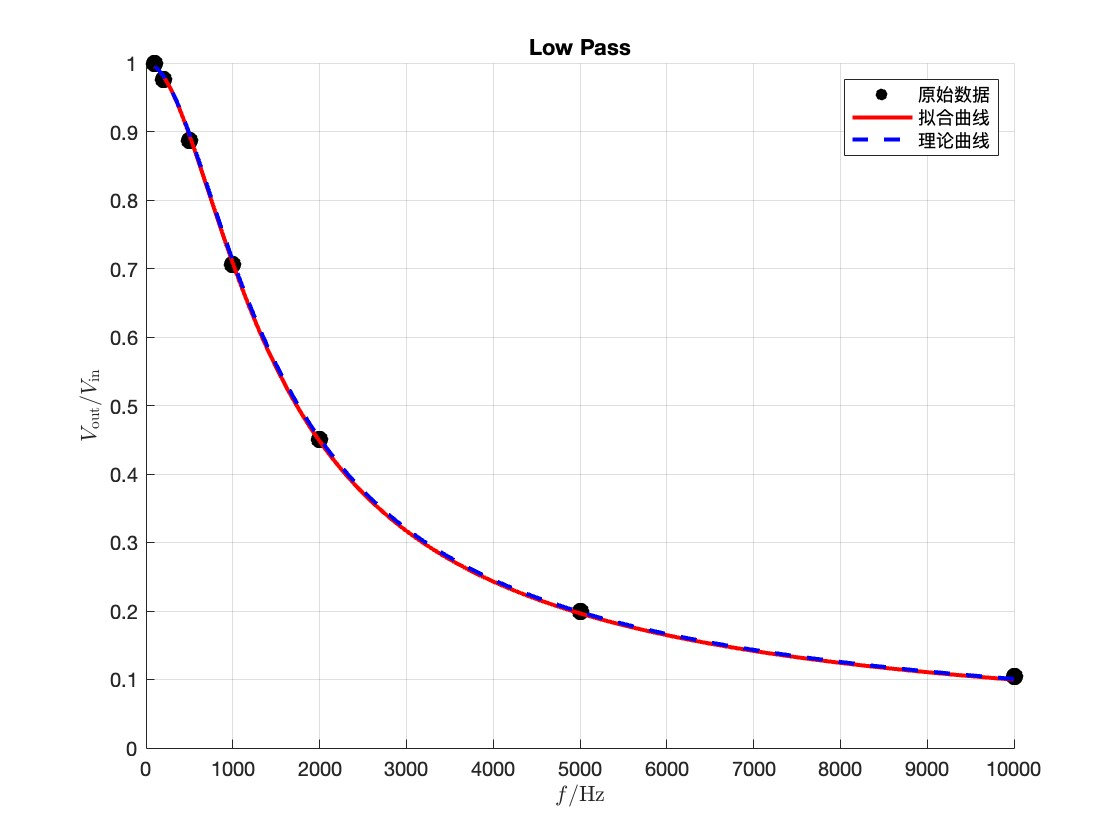
\includegraphics[width=\textwidth]{RC4L.jpg}
            \end{minipage}
            }
            \caption{$R=\qty{1.49}{\kohm}$，$C=\qty{105.4}{\nF}$}
        \end{figure}
        \begin{figure}[H]
            \centering
            \scalebox{0.8}{
            \begin{minipage}{0.45\textwidth}
                \centering
                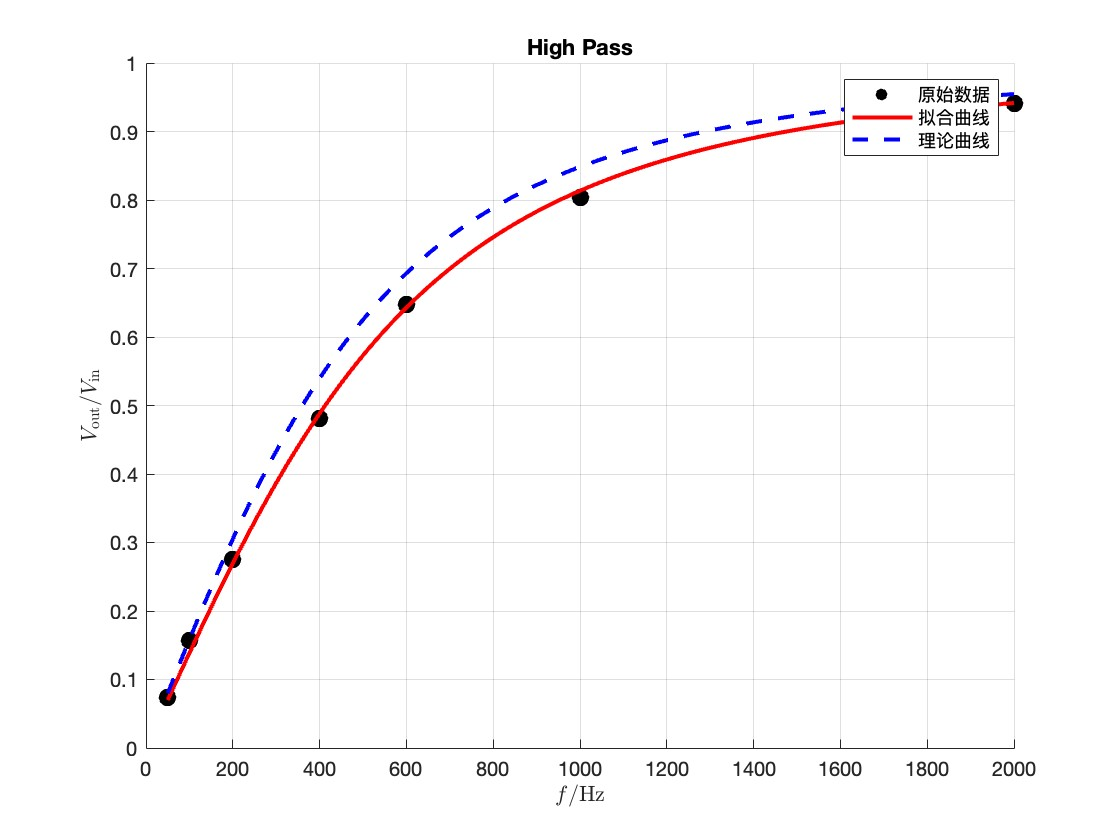
\includegraphics[width=\textwidth]{RC5H.jpg}
            \end{minipage}
            \begin{minipage}{0.45\textwidth}
                \centering
                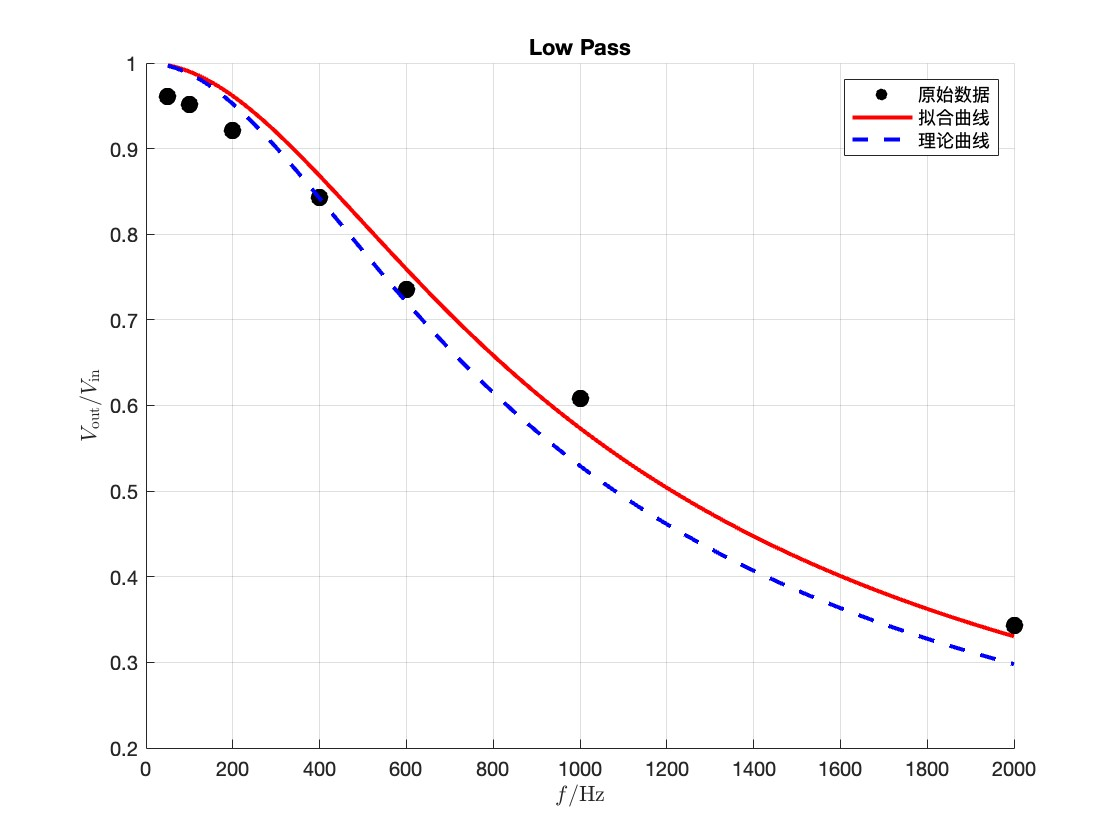
\includegraphics[width=\textwidth]{RC5L.jpg}
            \end{minipage}
            }
            \caption{$R=\qty{75}{\kohm}$，$C=\qty{3.4}{\nF}$}
        \end{figure}
    从图像可以看出，滤波电路对不同频率的实际响应基本符合理论预测。第五组实验与理论曲线偏离较多，可能原因是测量时信号发生器同时开启两个频道输出，经过对比发现同时启用两个频道会对输出频率和振幅产生较大影响，进而产生一定误差。另外，信号发生器和示波器存在内阻，会影响定值电阻阻值较小的情况下的实验结果。

    \item 使用LabVIEW与示波器通讯
    \\[1mm]
    如图，通过LabVIEW界面，可以实现示波器波形的监测以及参数的测量
    \begin{figure}[H]
            \centering
            \scalebox{0.9}{
            \begin{minipage}{0.45\textwidth}
                \centering
                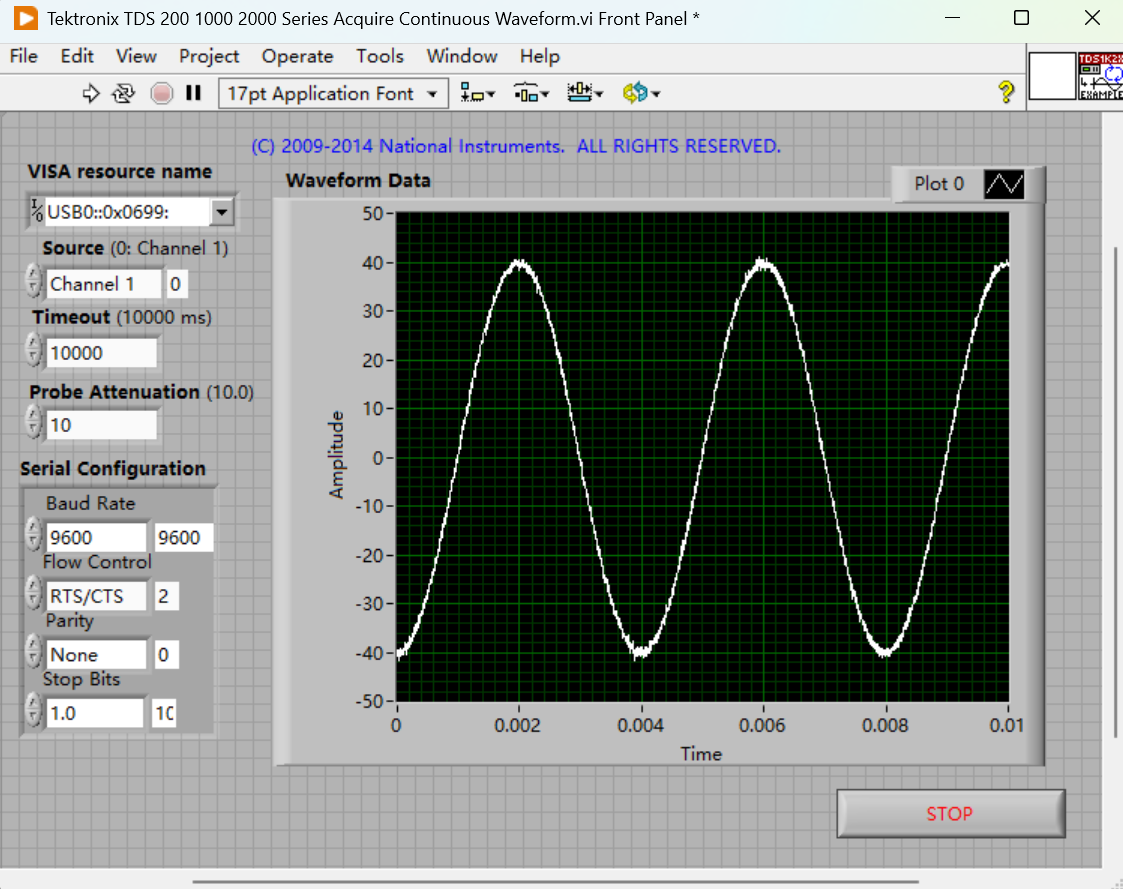
\includegraphics[width=\textwidth]{Wave1-2.PNG}
            \end{minipage}
            \begin{minipage}{0.45\textwidth}
                \centering
                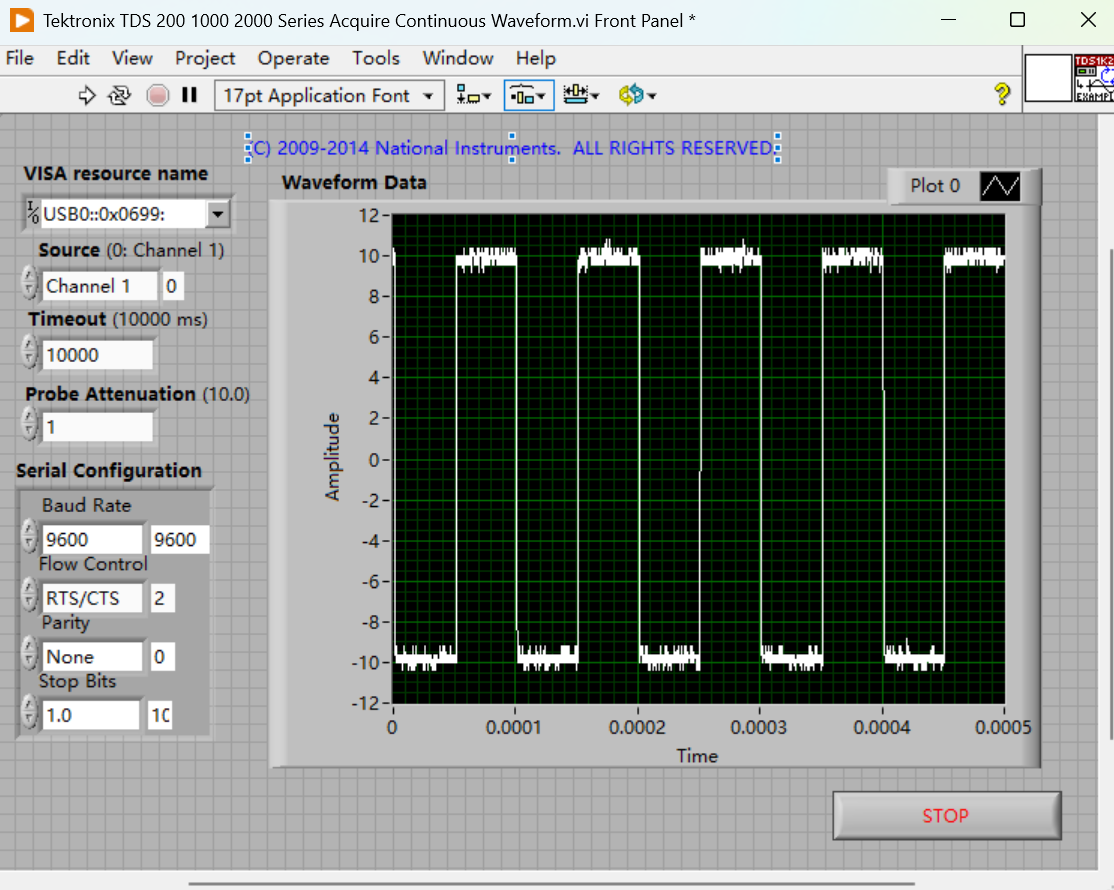
\includegraphics[width=\textwidth]{Wave2-2.PNG}
            \end{minipage}
            }
            \caption{LabVIEW与示波器通讯界面}
        \end{figure}

    \item 温度监测电路
    \\[1mm]
    电路如图1所示，其中定值电阻$R^*=\qty{9.9}{\kohm}$，热敏电阻$B=\qty{3380}{\K}$。将NI DAQ接入LabVIEW，并用LabVIEW程序处理。首先建立热敏电阻$R_\text{T}$的工作曲线：将热敏电阻整体浸入冰水混合物，使用LabVIEW测得$V = \qty{2.422}{\V}$，计算可得$R_0 = \qty{24.5}{\kohm}$。确定参数后使用LabVIEW程序以每秒一次的频率采集电压信号，处理后以摄氏度和华氏度两种标度输出温度。
    \begin{figure}[H]
        \centering
        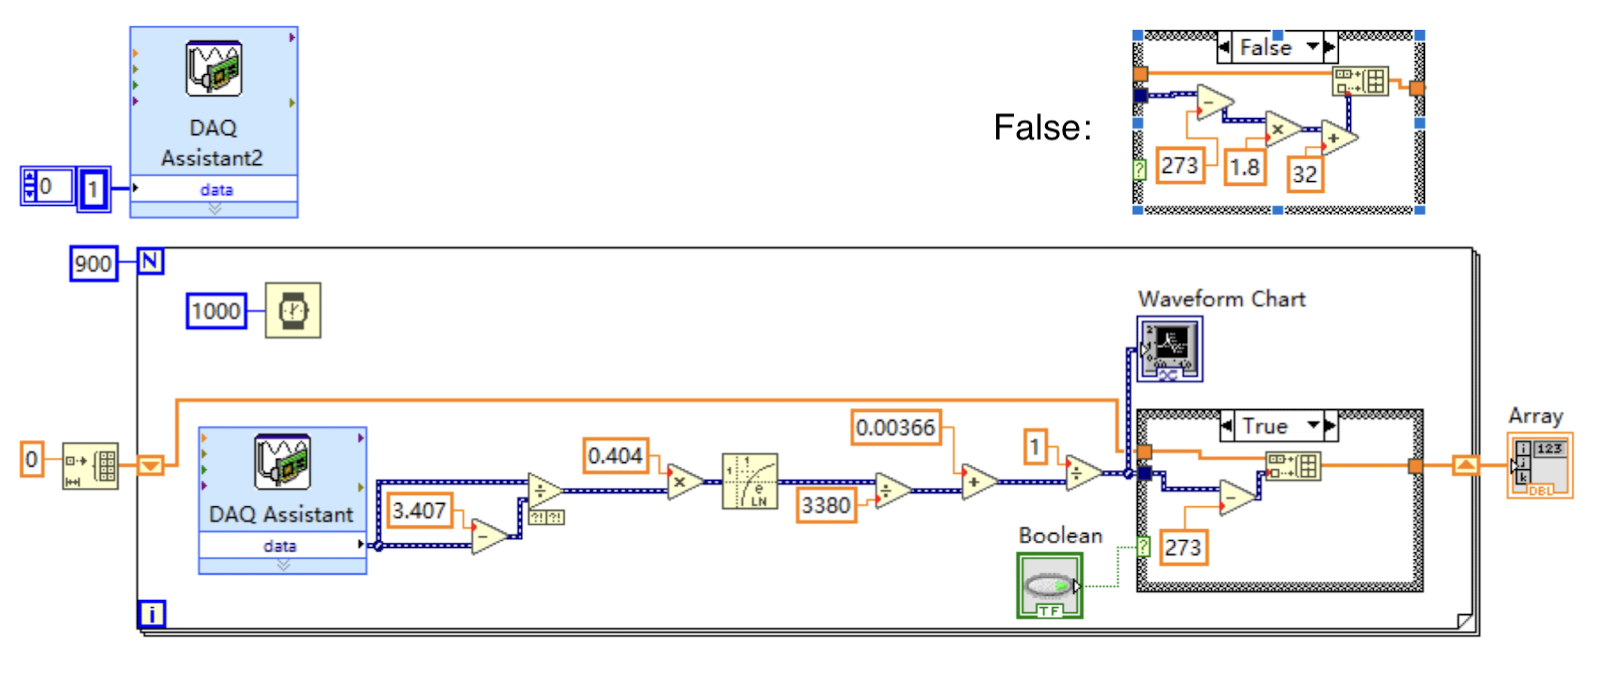
\includegraphics[width=0.7\linewidth]{LabVIEW.png}
        \caption{LabVIEW程序}
    \end{figure}
    使用该程序记录15分钟内温度变化，绘图得到：
    \begin{figure}[H]
        \centering
        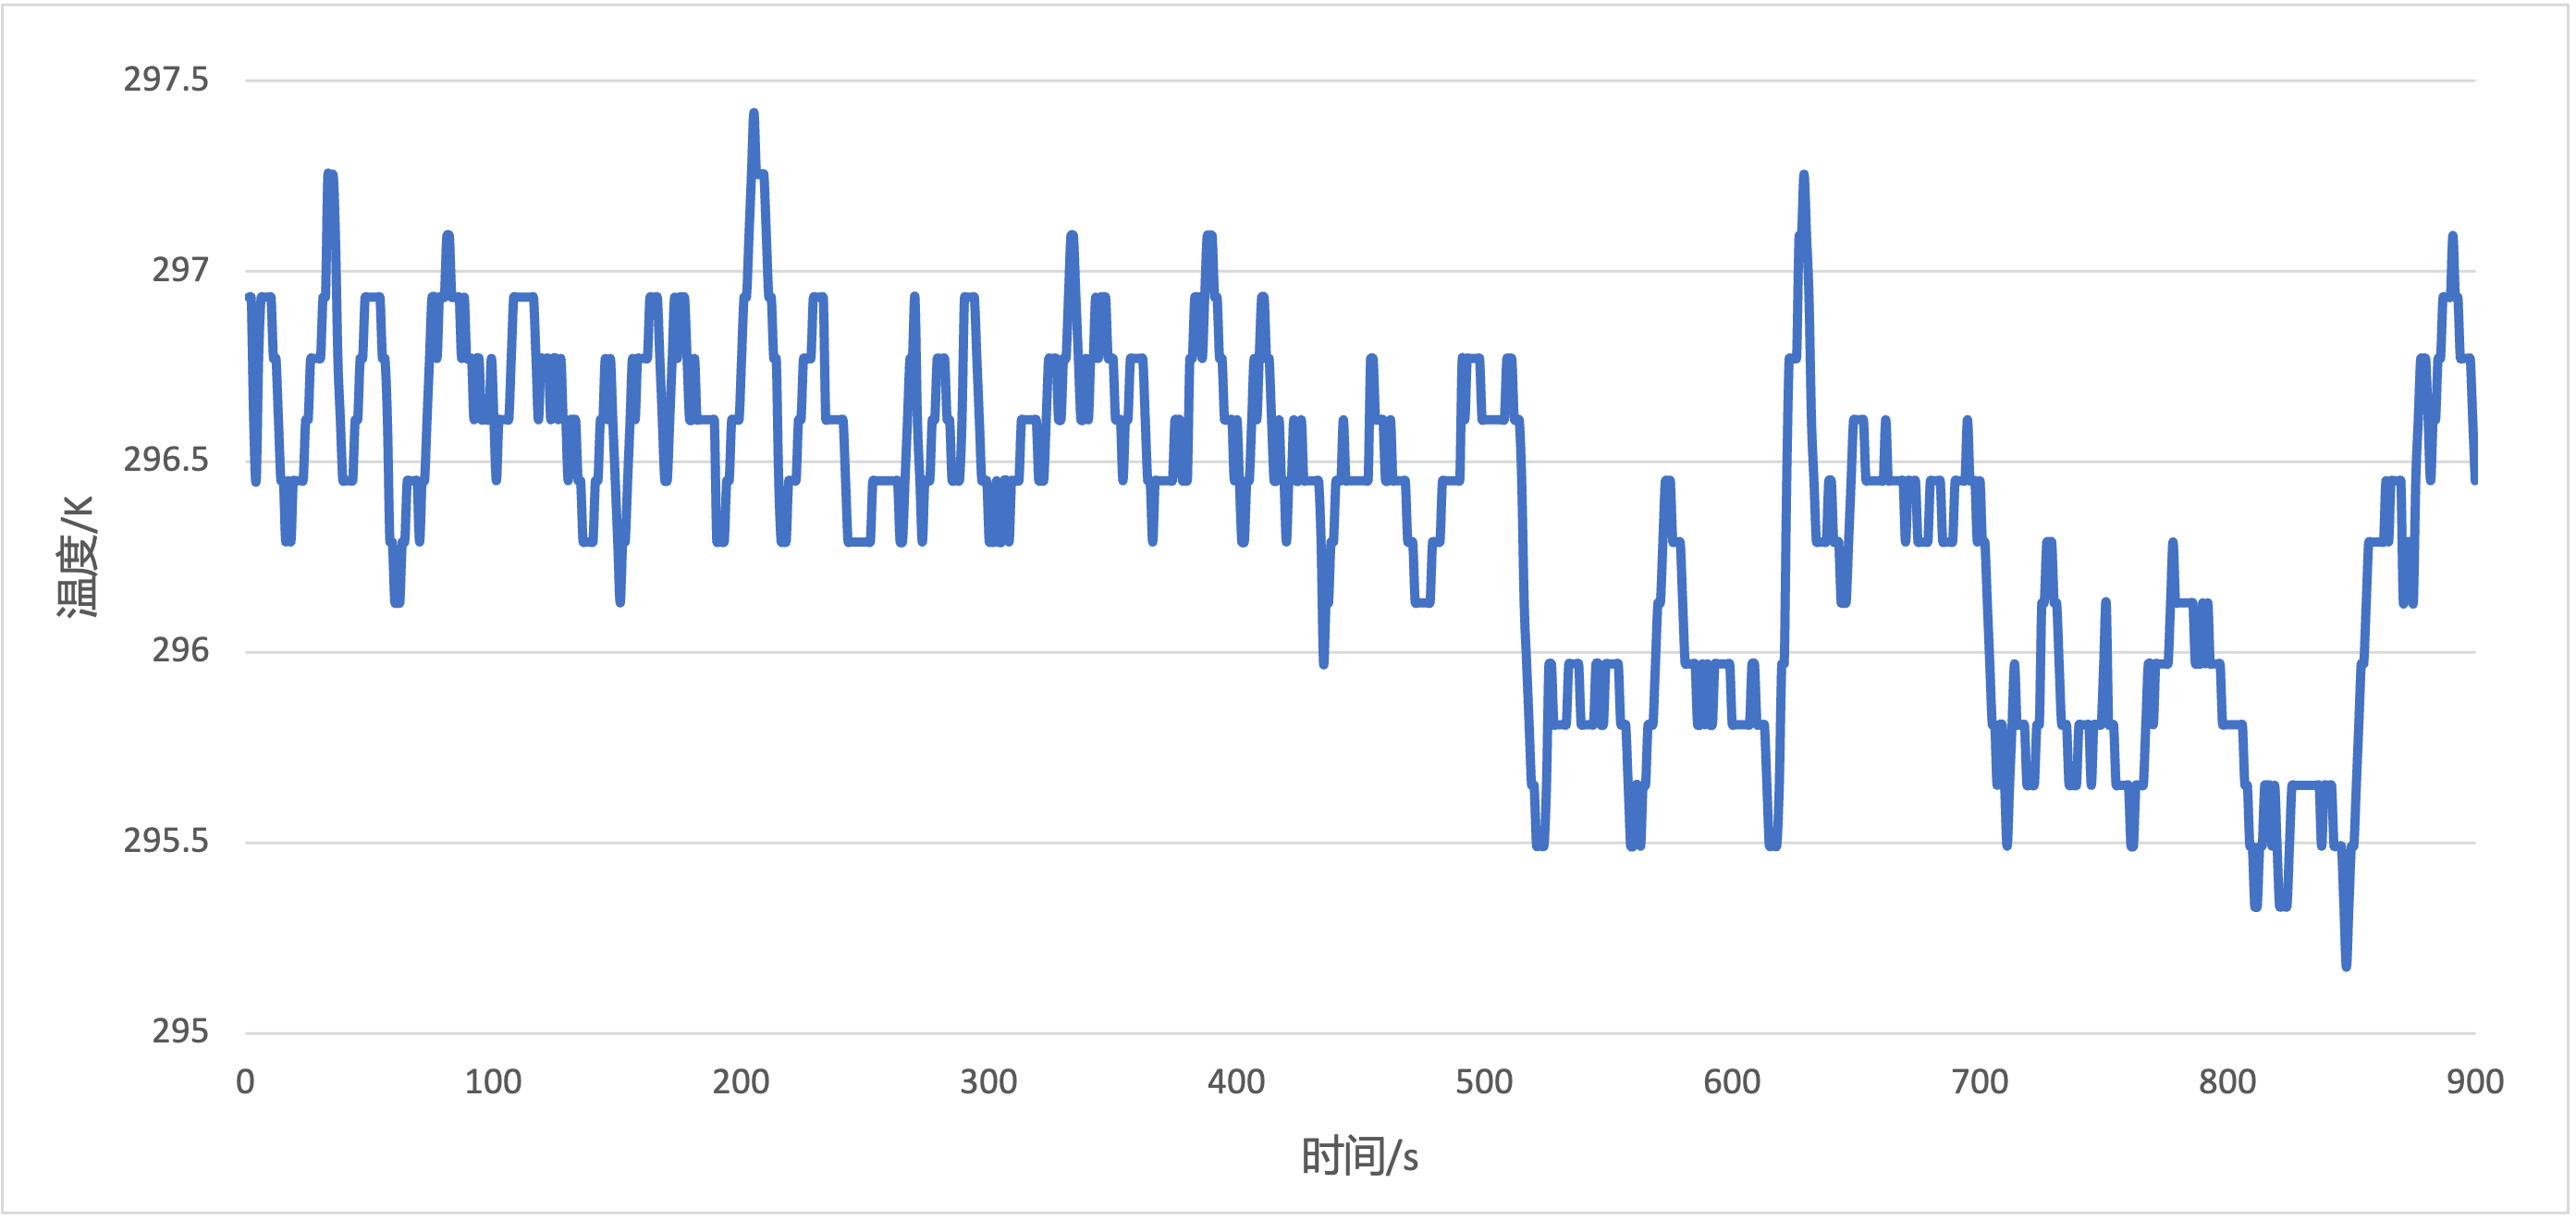
\includegraphics[width=0.7\linewidth]{Temp vs Time.png}
        \caption{温度-时间图像}
    \end{figure}
    本实验的误差主要来自于：未考虑DAQ元件的内阻以及DAQ输出电平的不稳定性；热敏电阻可能会略偏离已知的工作曲线：本实验仅测量了0摄氏度时的阻值，并用已知的$B$来校准工作曲线，这种方法未必能精确校准；环境中的干扰因素也会干扰热敏电阻附近的温度，使之偏离室温。
    \end{enumerate}
    

\end{enumerate}
\end{document}